\documentclass[pdflatex,compress,mathserif]{beamer}

%\usetheme[dark,framenumber,totalframenumber]{ElektroITK}
\usetheme[darktitle,framenumber,totalframenumber]{ElektroITK}

\usepackage[utf8]{inputenc}
\usepackage[T1]{fontenc}
\usepackage{lmodern}
\usepackage[bahasai]{babel}
\usepackage{amsmath}
\usepackage{amsfonts}
\usepackage{amssymb}
\usepackage{graphicx}
\usepackage{multicol}
\usepackage{lipsum}
\usefonttheme[onlymath]{serif}

\newcommand*{\Scale}[2][4]{\scalebox{#1}{$#2$}}%

\setbeamertemplate{caption}[numbered]

\title{MATEMATIKA DASAR}
\subtitle{Operasi Bilangan Real}

\author{Mifta Nur Farid}

\begin{document}

% ----------------------------------------------------------------------------
% *** Titlepage <<<
% ----------------------------------------------------------------------------
\maketitle
% ----------------------------------------------------------------------------
% *** END of Titlepage >>>
% ----------------------------------------------------------------------------

\section{Bilangan Real}

\begin{frame}
\frametitle{Bilangan Real}
	\begin{center}
		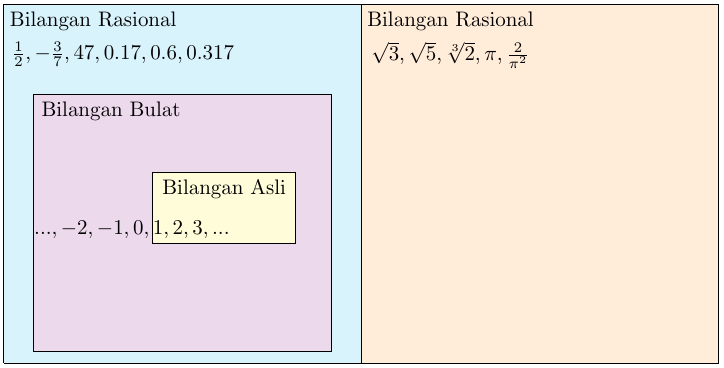
\includegraphics[width=0.7\linewidth]{img/img01}
	\end{center}
	\begin{itemize}
		\item Himpunan bilangan real: kumpulan dari himpunan bilangan rasional dan irasional
		\item Notasi bilangan real: $\mathbb{R}$
	\end{itemize}
\end{frame}

\begin{frame}{Bilangan Real}
	\begin{itemize}
		\item Setiap bilangan real dapat dinyatakan dalam bentuk desimal.
		\item Jika bilangan tersebut merupakan bilangan rasional, maka akan terdapat desimal yang berulang, sebagai contoh berikut
	\end{itemize}
	\begin{center}
		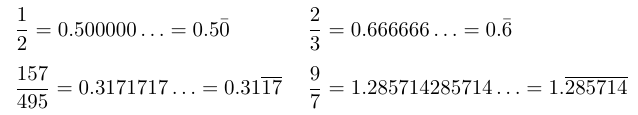
\includegraphics[width=0.8\linewidth]{img/img02}
	\end{center}
\end{frame}

\begin{frame}{Bilangan Real}
	\begin{itemize}
		\item Sedangkan jika bilangan merupakan bilangan irasional, desimal bilangan tersebut tidak akan berulang, seperti
	\end{itemize}
	\begin{center}
		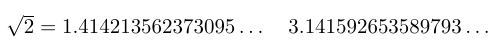
\includegraphics[width=0.7\linewidth]{img/img03}
	\end{center}
\end{frame}

\begin{frame}{Bilangan Real}
	\begin{itemize}
		\item Jika hanya dipotong sampai beberapa digit desimal, bilangan tersebut dinyatakan sebagai aproksimasi nilai tersebut.
	\end{itemize}
	\begin{center}
		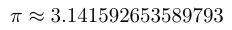
\includegraphics[width=0.4\linewidth]{img/img04}
	\end{center}
\end{frame}

\begin{frame}
	\frametitle{Sifat Bilangan Real}
	\begin{center}
		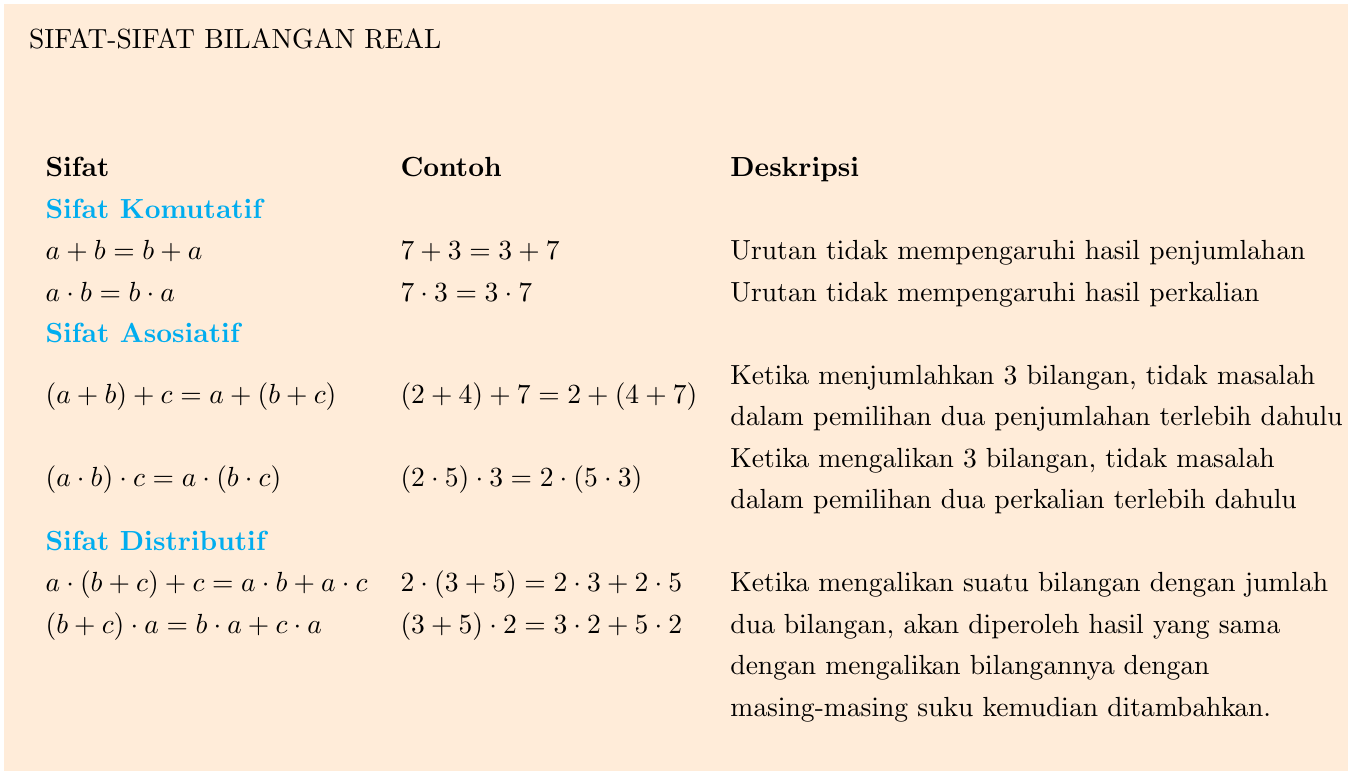
\includegraphics[width=\linewidth]{img/img05}
	\end{center}
\end{frame}

\begin{frame}{Sifat Bilangan Real}
	\begin{center}
		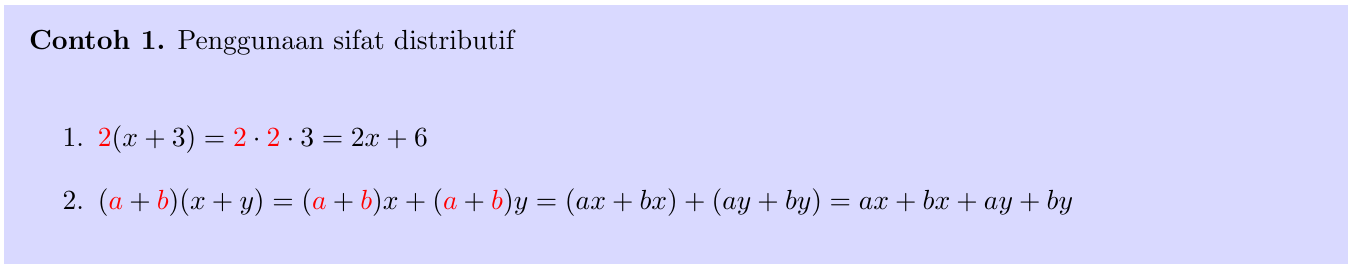
\includegraphics[width=\linewidth]{img/img06}
	\end{center}
\end{frame}

\begin{frame}
	\frametitle{Penjumlahan dan Pengurangan}
	\begin{center}
		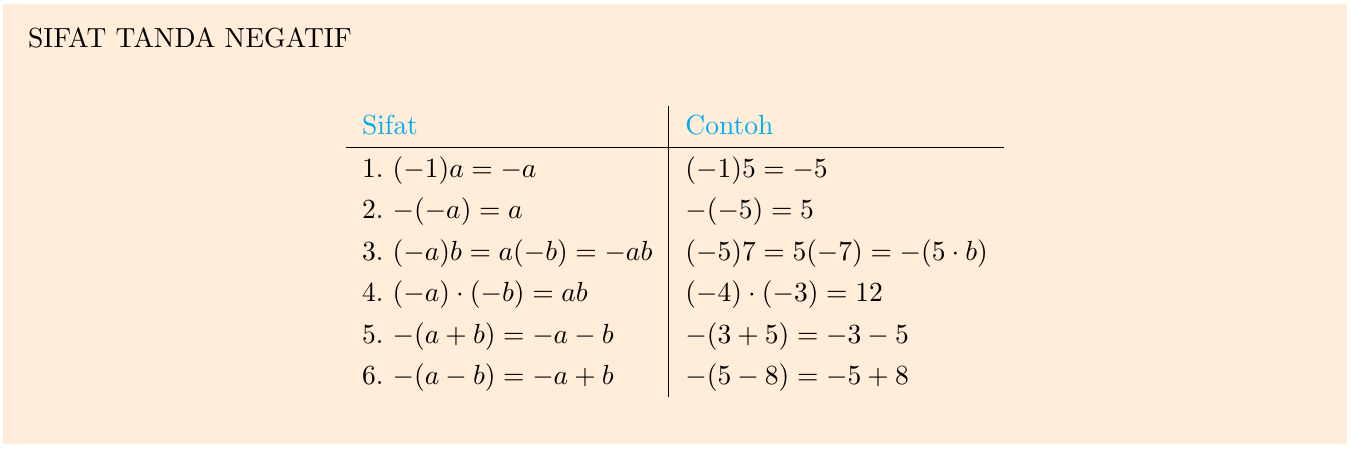
\includegraphics[width=\linewidth]{img/img07}
	\end{center}
\end{frame}

\begin{frame}{Penjumlahan dan Pengurangan}
	\begin{center}
		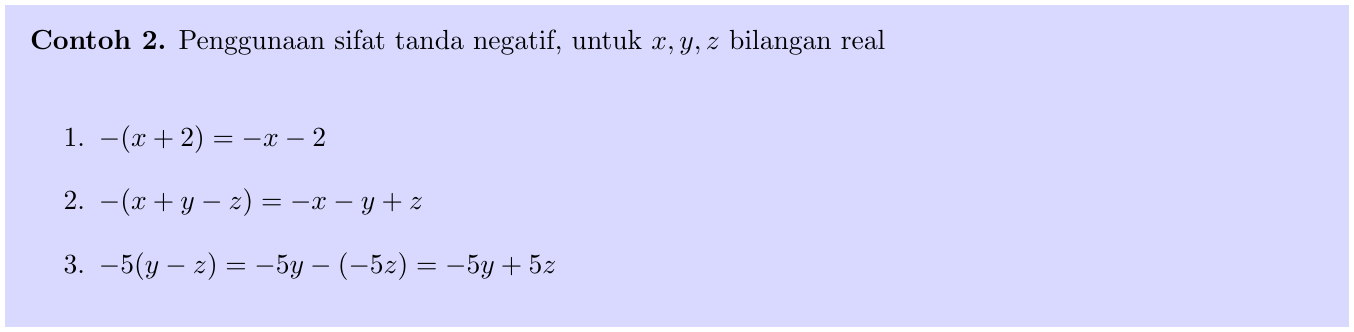
\includegraphics[width=\linewidth]{img/img08}
	\end{center}
\end{frame}

\begin{frame}
	\frametitle{Perkalian dan Pembagian}
	\begin{center}
		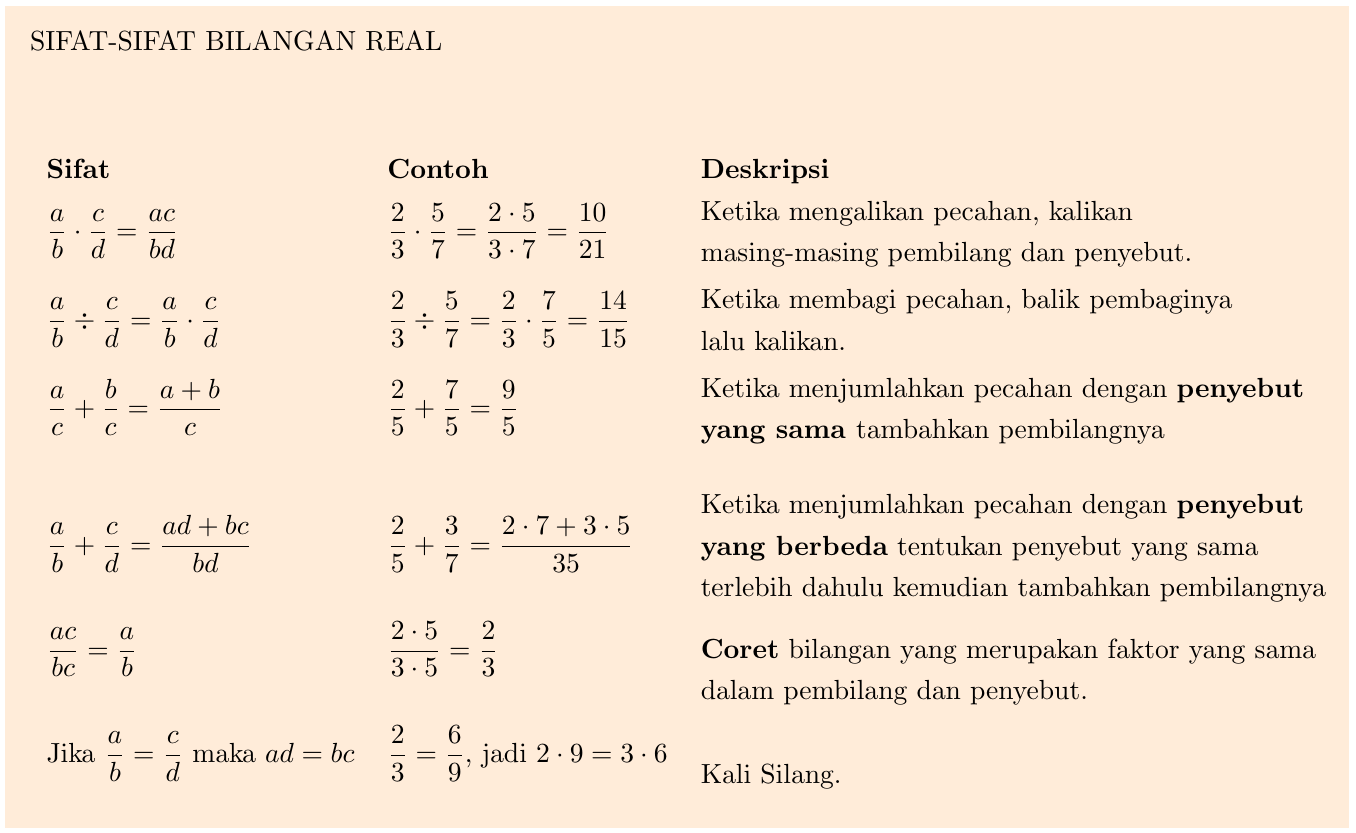
\includegraphics[width=\linewidth]{img/img09}
	\end{center}
\end{frame}

\begin{frame}{Perkalian dan Pembagian}
	\begin{center}
		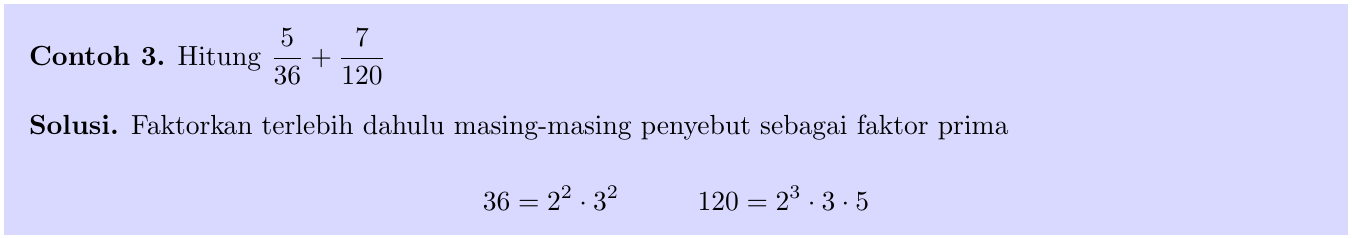
\includegraphics[width=\linewidth]{img/img10}
		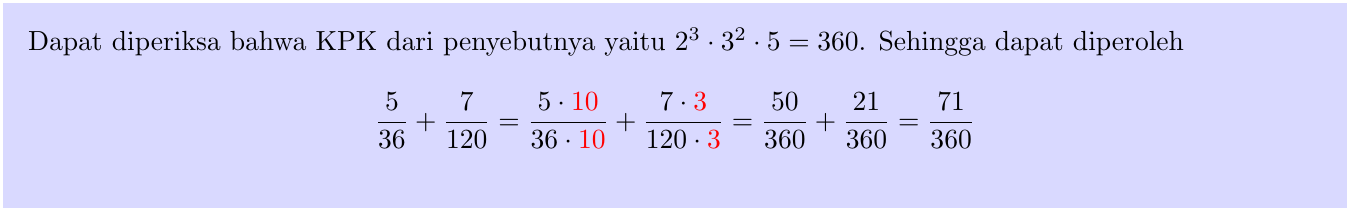
\includegraphics[width=\linewidth]{img/img11}
	\end{center}
\end{frame}

\begin{frame}
	\frametitle{Garis Bilangan}
	\begin{itemize}
		\item Bilangan real dapat dinyatakan sebagai titik dalam garis sebagai berikut
	\end{itemize}
	\begin{center}
		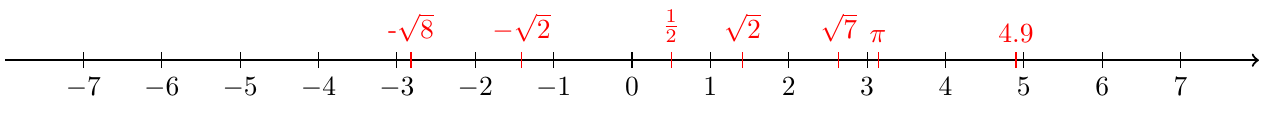
\includegraphics[width=\linewidth]{img/img12}
	\end{center}
\end{frame}

\begin{frame}
	\frametitle{Himpunan dan Interval}
	\begin{itemize}
		\item Suatu himpuan adalah koleksi dari objek, objeknya dari himpunan disebut sebagai anggota.
		\item Jika $S$ adalah himpunan, notasi $a \in S$ berarti bahwa a merupakan anggota dari $S$, dan notasi $b \notin S$ berarti bahwa $b$ bukan anggota dari $S$.
		\item "A merupakan himpunan seluruh x sehingga x berada diantara 0 dan 7"
		\begin{itemize}
			\item[] $A = \{1, 2, 3, 4, 5, 6\}$
			\item[] $A = \{x|x \text{ bilangan bulat dan } 0 < x < 7\}$
		\end{itemize}
	\end{itemize}
\end{frame}

\begin{frame}{Himpunan dan Interval}
	\begin{itemize}
		\item Jika S dan T merupakan himpunan, \textbf{gabungan} kedua himpunan tersebut S $\cup$ T adalah himpunan yang terdiri dari seluruh anggotanya di S atau T (atau keduanya).
		\item \textbf{Irisan} dari himpunan S dan T adalah himpunan S $\cap$ T yang terdiri dari seluruh anggota yang keduanya berada di S dan T . Dengan kata lain, S $\cap$ T terdiri dari anggota-anngota yang keduanya berada pada himpunan S dan T .
		\item \textbf{Himpunan kosong} yang dinyatakan sebagai $\emptyset$ merupakan himpunan yang tidak mempunyai anggota.
	\end{itemize}
\end{frame}

\begin{frame}{Himpunan dan Interval}
	\begin{center}
		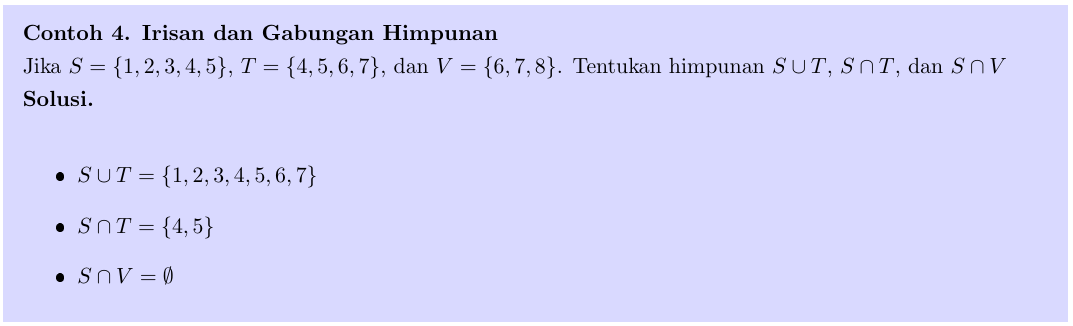
\includegraphics[width=\linewidth]{img/img13}
	\end{center}
\end{frame}

\begin{frame}{Himpunan dan Interval}
	\begin{itemize}
		\item Interval terbuka
		\begin{center}
			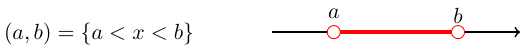
\includegraphics[width=\linewidth]{img/img14}
		\end{center}
		\item Interval tertutup
		\begin{center}
			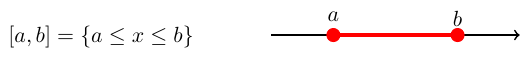
\includegraphics[width=\linewidth]{img/img15}
		\end{center}
	\end{itemize}
\end{frame}

\begin{frame}{Himpunan dan Interval}
	\begin{center}
		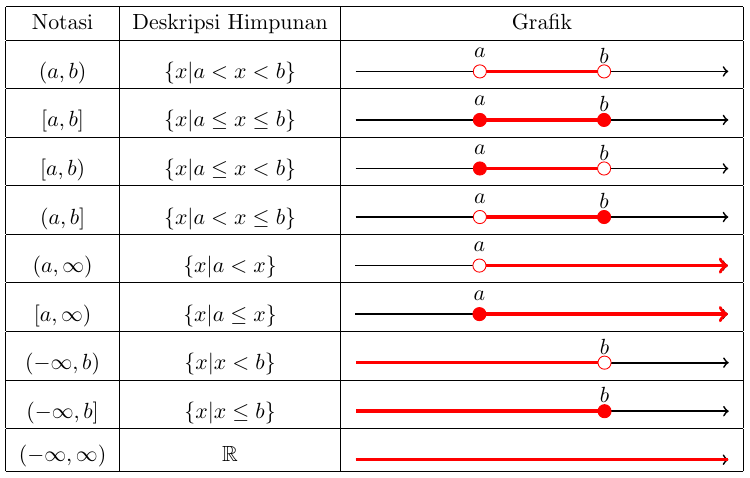
\includegraphics[width=0.9\linewidth]{img/img16}
	\end{center}
\end{frame}

\begin{frame}{Himpunan dan Interval}
	\begin{center}
		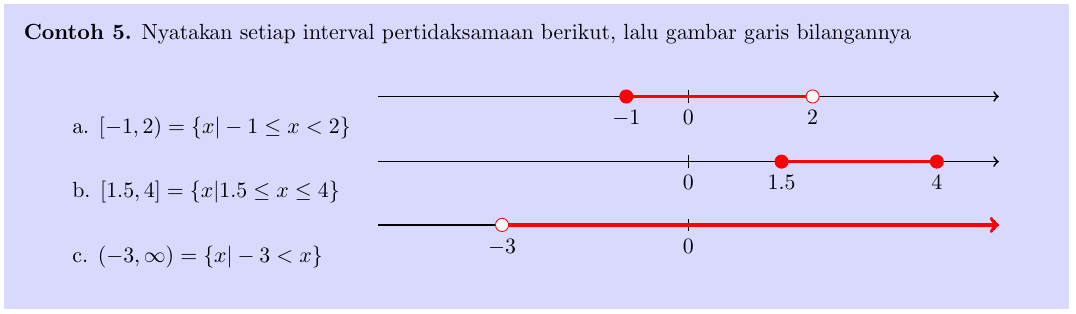
\includegraphics[width=\linewidth]{img/img17}
	\end{center}
\end{frame}

\begin{frame}{Himpunan dan Interval}
	\begin{center}
		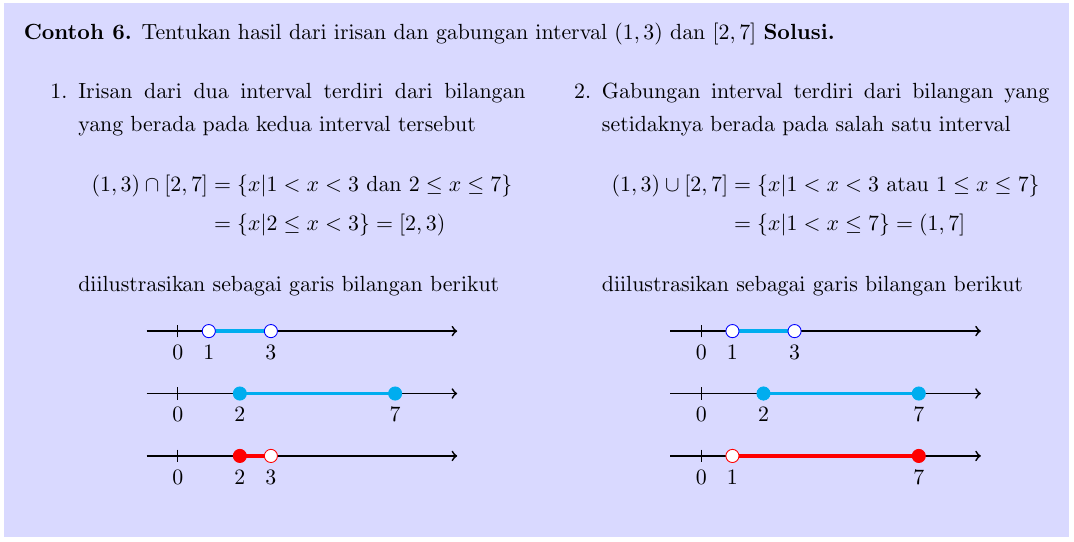
\includegraphics[width=\linewidth]{img/img18}
	\end{center}
\end{frame}

\begin{frame}
	\frametitle{Ekspresi bentuk Aljabar}
	\begin{itemize}
		\item Suatu \textbf{monomial} merupakan ekspresi aljabar dengan bentuk $ax^k$ dengan $a$ bilangan real dan $k$ merupakan bilangan bulat tidak negatif.
	\end{itemize}
\end{frame}

\begin{frame}{Ekspresi bentuk Aljabar}
	\begin{center}
		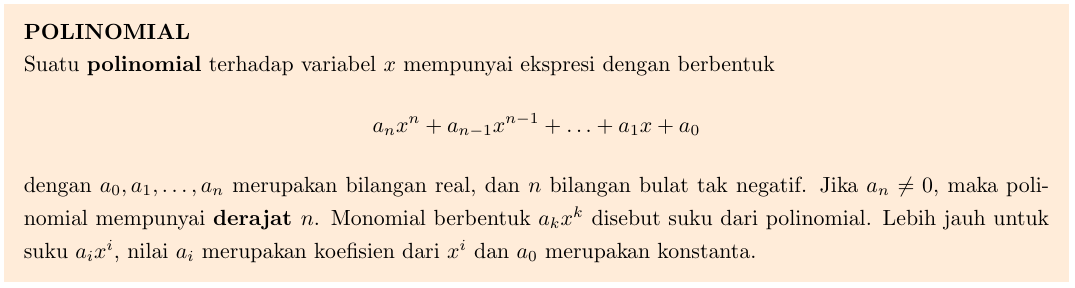
\includegraphics[width=\linewidth]{img/img19}
	\end{center}
\end{frame}

\begin{frame}{Ekspresi bentuk Aljabar}
	\begin{center}
		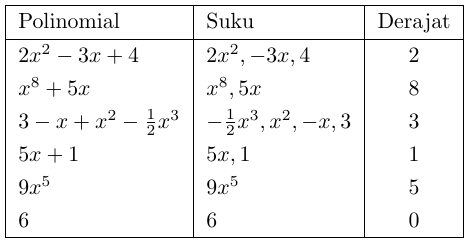
\includegraphics[width=0.7\linewidth]{img/img20}
	\end{center}
\end{frame}

\begin{frame}
	\frametitle{Operasi Penjumlahan dan\\Pengurangan Polinomial}
	\begin{center}
		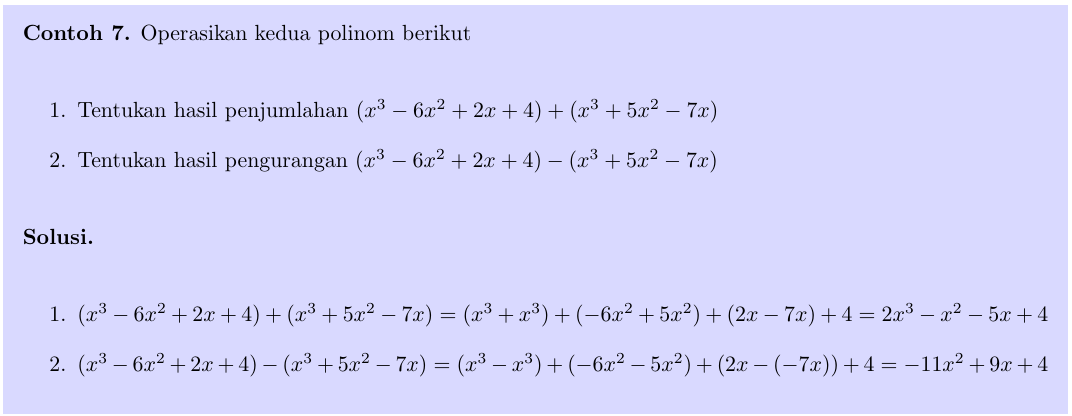
\includegraphics[width=\linewidth]{img/img21}
	\end{center}
\end{frame}

\begin{frame}
	\frametitle{Operasi Perkalian pada Polinomial}
	\begin{center}
		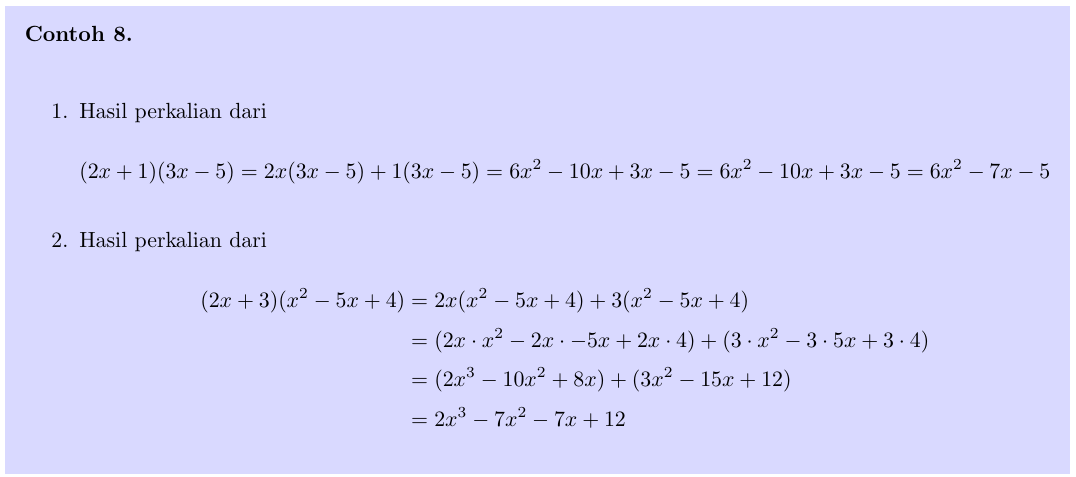
\includegraphics[width=\linewidth]{img/img22}
	\end{center}
\end{frame}

\begin{frame}{Operasi Perkalian pada Polinomial}
	\begin{itemize}
		\item Beberapa bentuk perkalian khusus dari suatu ekspresi aljabar berikut sering muncul, sehingga lebih baik perlu dihafalkan
	\end{itemize}
	\begin{center}
		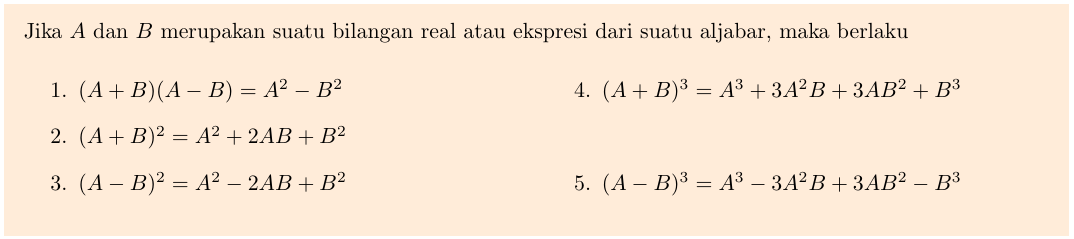
\includegraphics[width=\linewidth]{img/img23}
	\end{center}
\end{frame}

\begin{frame}{Operasi Perkalian pada Polinomial}
	\begin{center}
		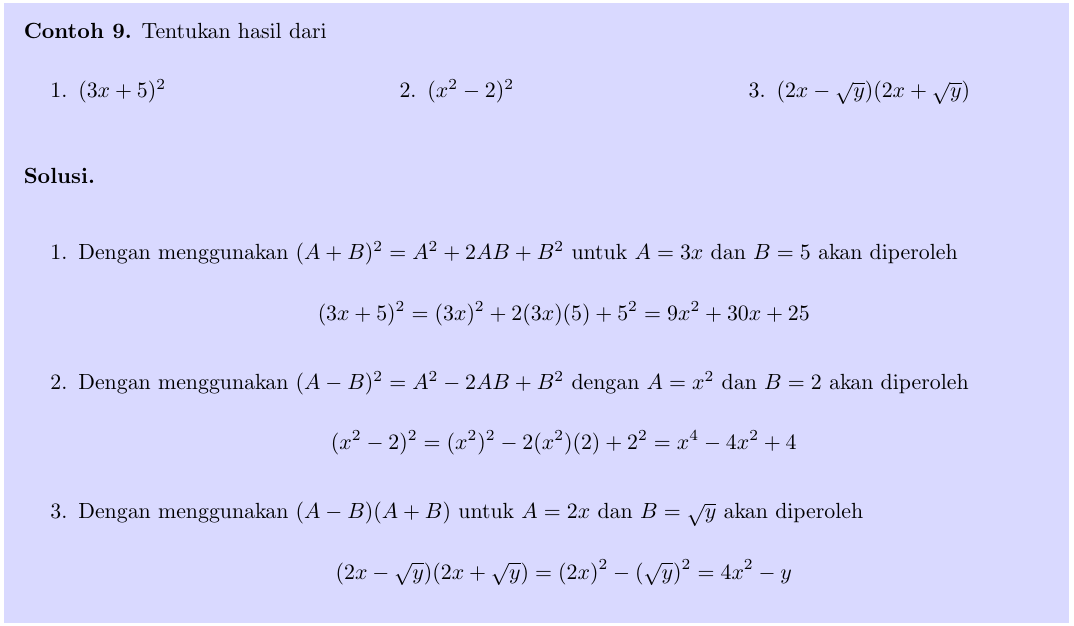
\includegraphics[width=\linewidth]{img/img24}
	\end{center}
\end{frame}

\begin{frame}
	\frametitle{Pemfaktoran}
	\begin{itemize}
		\item Perhatikan bahwa $(x - 2)(x + 2) = x^2 - 4$ maka dapat disebut bahwa $(x - 2)$ dan $(x + 2)$ merupakan faktor dari $x^2 - 4$.
		\item Dalam pemfaktoran biasanya diperlukan menentukan faktor persekutuan terbesar (FPB) dari koefisien dan pangkat terendah dari suatu bentuk $x^k$, atau juga bisa melihat dari faktor yang sama.
	\end{itemize}
\end{frame}

\begin{frame}{Pemfaktoran}
	\begin{center}
		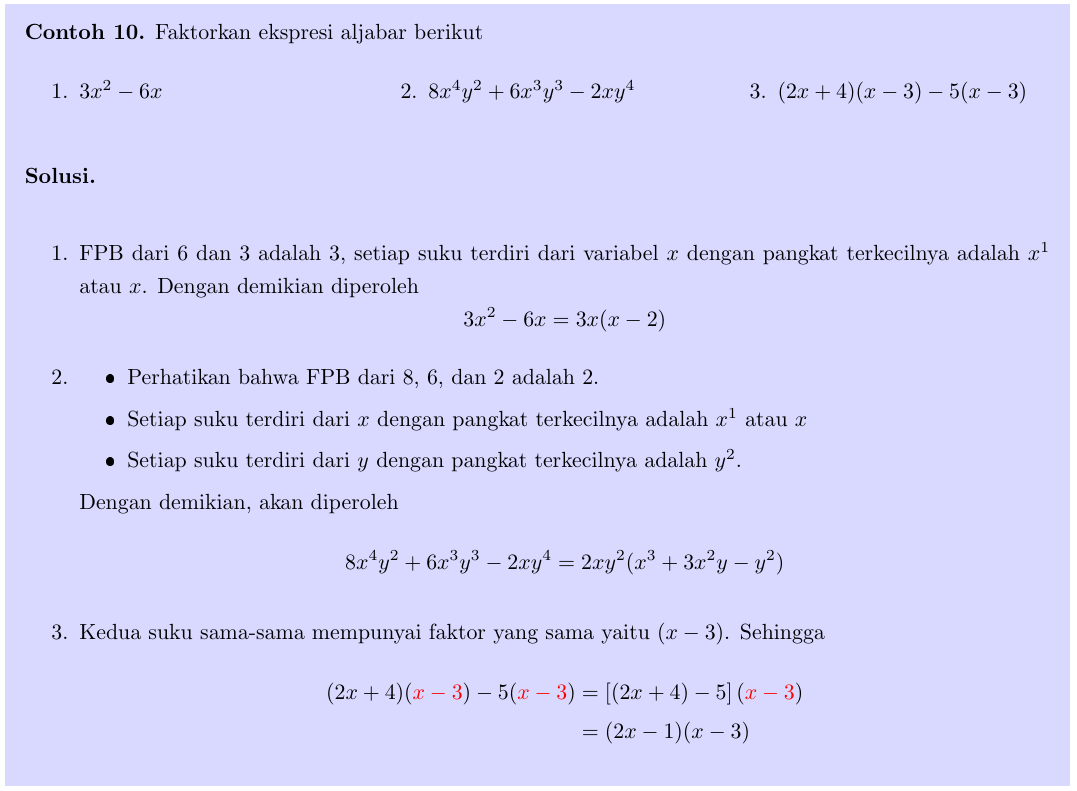
\includegraphics[width=0.9\linewidth]{img/img25}
	\end{center}
\end{frame}

\begin{frame}{Pemfaktoran}
	\begin{center}
		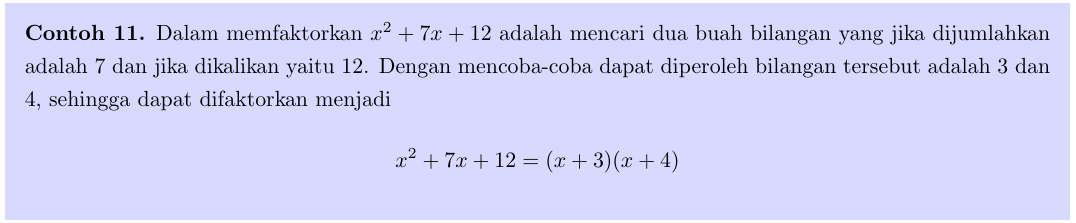
\includegraphics[width=\linewidth]{img/img26}
	\end{center}
\end{frame}

\begin{frame}{Pemfaktoran}
	\begin{center}
		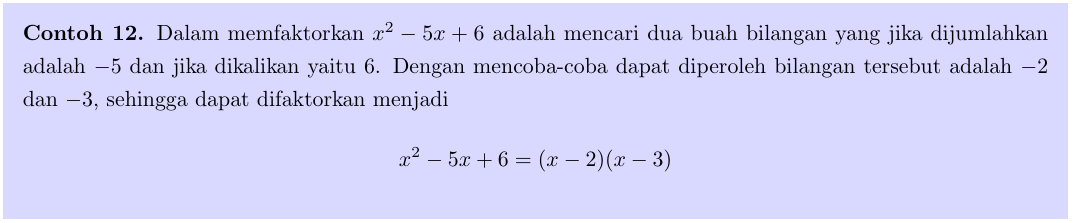
\includegraphics[width=\linewidth]{img/img27}
	\end{center}
\end{frame}

\begin{frame}{Pemfaktoran}
	\begin{center}
		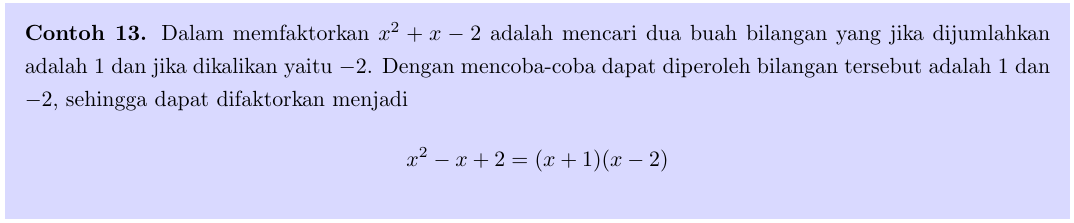
\includegraphics[width=\linewidth]{img/img28}
	\end{center}
\end{frame}

\begin{frame}{Pemfaktoran}
	\begin{center}
		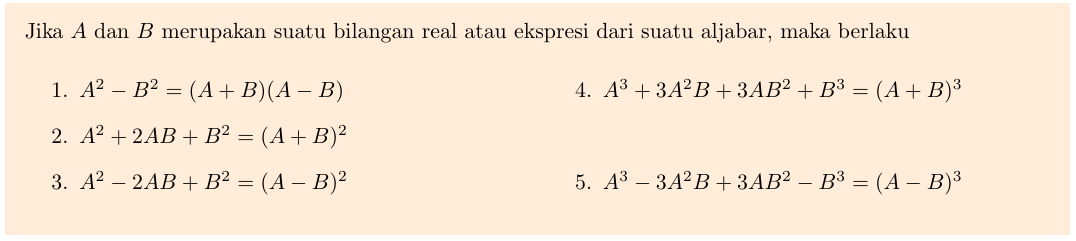
\includegraphics[width=\linewidth]{img/img29}
	\end{center}
\end{frame}

\begin{frame}{Pemfaktoran}
	\begin{center}
		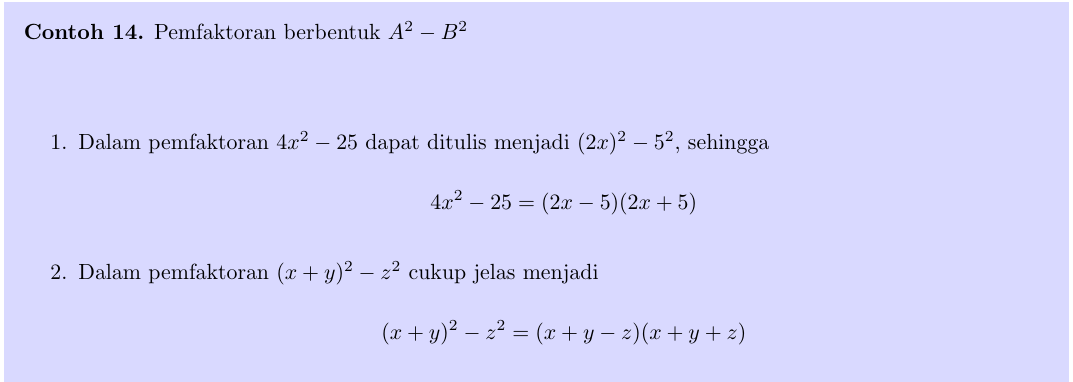
\includegraphics[width=\linewidth]{img/img30}
	\end{center}
\end{frame}

\begin{frame}{Pemfaktoran}
	\begin{center}
		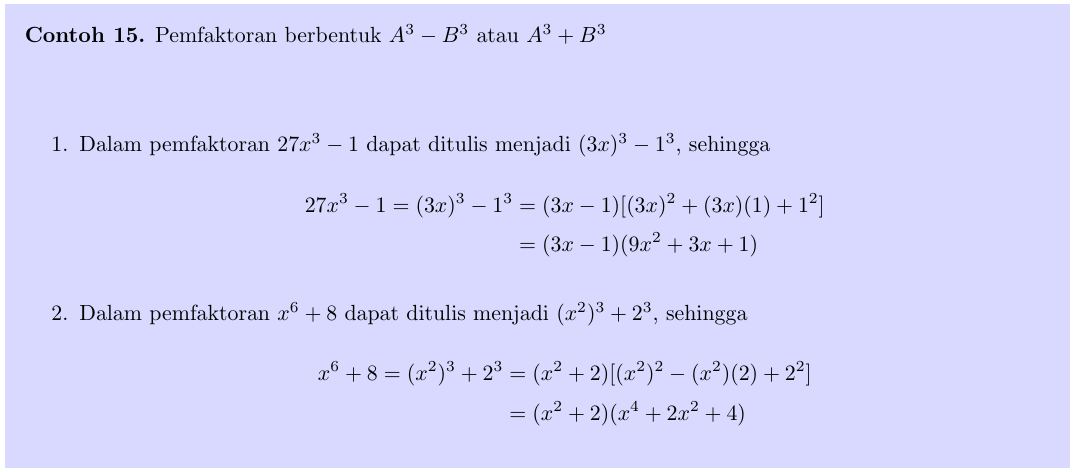
\includegraphics[width=\linewidth]{img/img31}
	\end{center}
\end{frame}

\begin{frame}
	\frametitle{Domain dari Ekspresi Aljabar}
	\begin{center}
		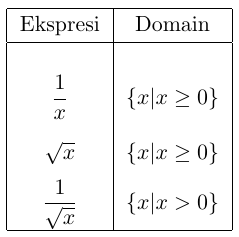
\includegraphics[width=0.5\linewidth]{img/img32}
	\end{center}
\end{frame}

\begin{frame}{Domain dari Ekspresi Aljabar}
	\begin{center}
		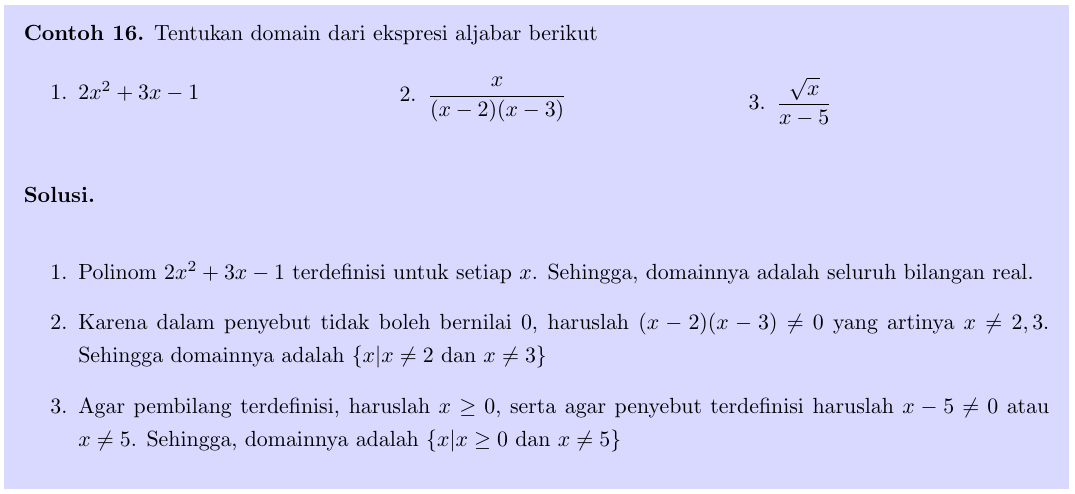
\includegraphics[width=\linewidth]{img/img33}
	\end{center}
\end{frame}

\begin{frame}
	\frametitle{Perkalian dan Pembagian Bentuk Ekspresi Rasional}
	\begin{center}
		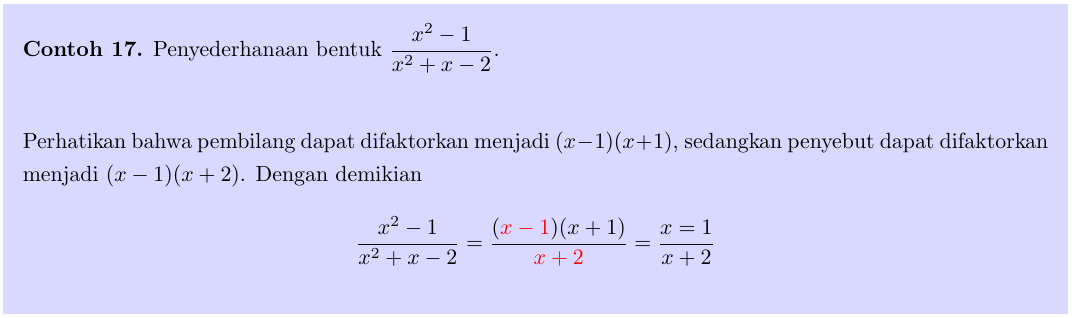
\includegraphics[width=\linewidth]{img/img34}
	\end{center}
\end{frame}

\begin{frame}{Perkalian dan Pembagian Bentuk Ekspresi Rasional}
	\begin{center}
		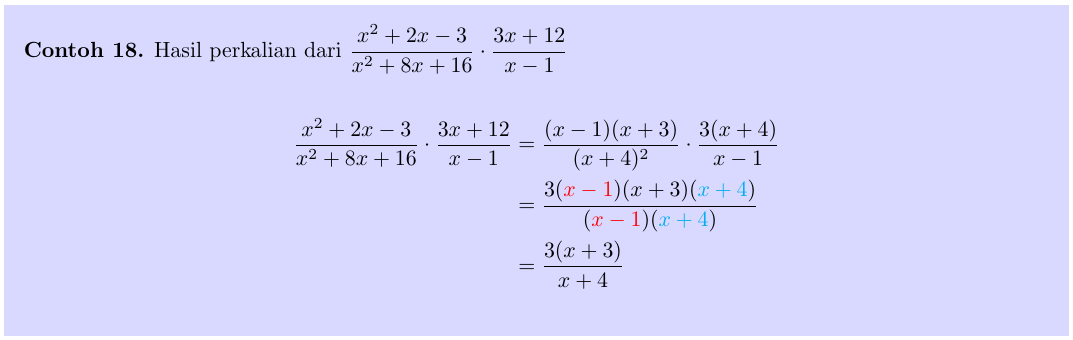
\includegraphics[width=\linewidth]{img/img35}
	\end{center}
\end{frame}

\begin{frame}{Perkalian dan Pembagian Bentuk Ekspresi Rasional}
	\begin{center}
		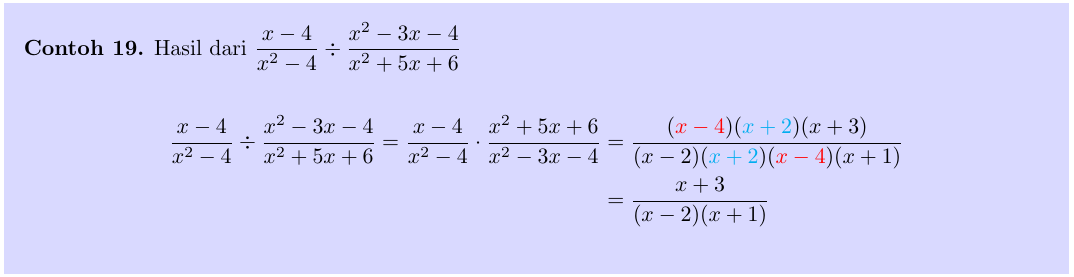
\includegraphics[width=\linewidth]{img/img36}
	\end{center}
\end{frame}

\begin{frame}
	\frametitle{Penjumlahan dan Perkalian Bentuk Ekspresi Rasional}
	\begin{itemize}
		\item Jika penyebutnya mempunyai bentuk yang sama, dapat digunakan operasi berikut
		\begin{equation*}
			\frac{A}{C} + \frac{B}{C} = \frac{A + B}{C}
		\end{equation*}
		\item Jika penyebut berbeda, maka dapat digunakan operasi berikut
		\begin{equation*}
			\frac{A}{B} + \frac{C}{D} = \frac{AD + BC}{BD}
		\end{equation*}
		\item Secara umum dalam operasi bentuk rasional jika penyebut tidak sama, dapat disamakan terlebih dahulu dengan memfaktorkan penyebut-penyebutnya lalu lihat ”KPK” dari kedua penyebutnya.
	\end{itemize}
\end{frame}

\begin{frame}{Penjumlahan dan Perkalian Bentuk Ekspresi Rasional}
	\begin{center}
		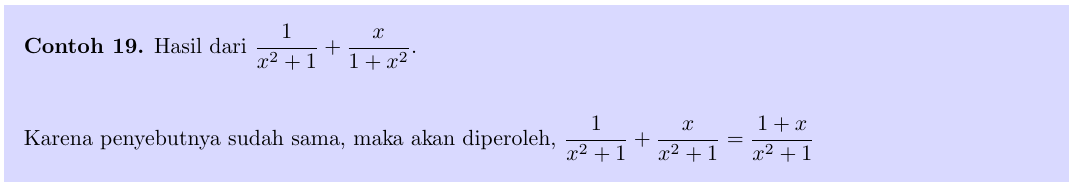
\includegraphics[width=\linewidth]{img/img37}
	\end{center}
\end{frame}

\begin{frame}{Penjumlahan dan Perkalian Bentuk Ekspresi Rasional}
	\begin{center}
		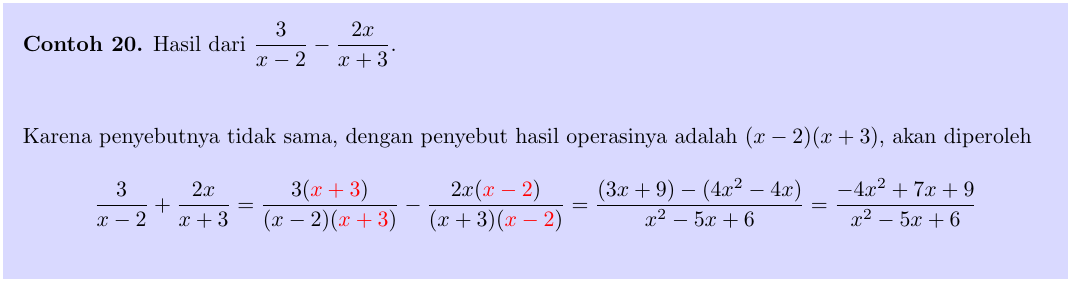
\includegraphics[width=\linewidth]{img/img38}
	\end{center}
\end{frame}

\begin{frame}{Penjumlahan dan Perkalian Bentuk Ekspresi Rasional}
	\begin{center}
		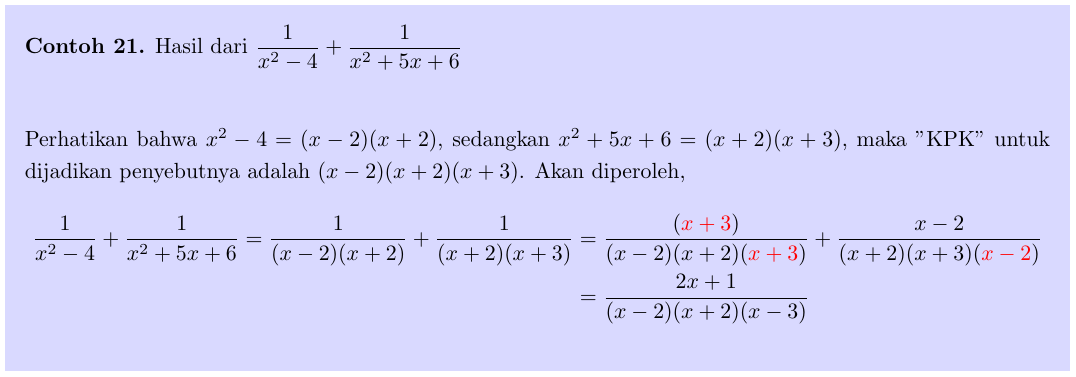
\includegraphics[width=\linewidth]{img/img39}
	\end{center}
\end{frame}

\begin{frame}
	\frametitle{Merasionalkan Bentuk Rasional}
	\begin{center}
		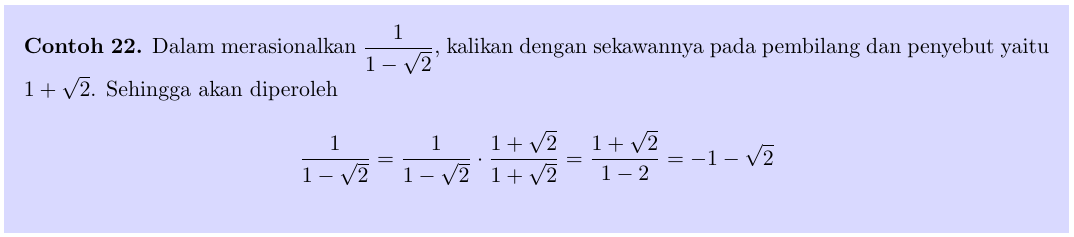
\includegraphics[width=\linewidth]{img/img40}
	\end{center}
\end{frame}

\begin{frame}{Merasionalkan Bentuk Rasional}
	\begin{center}
		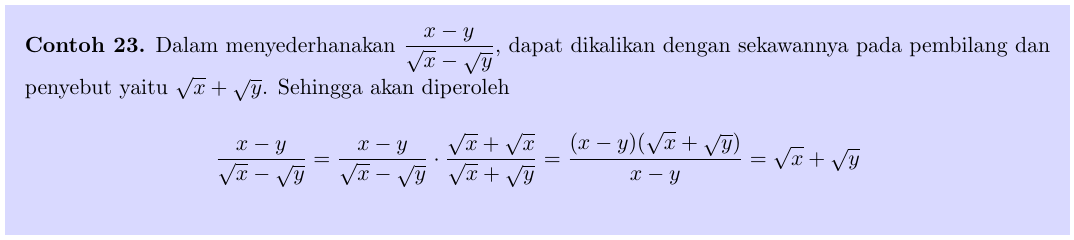
\includegraphics[width=\linewidth]{img/img41}
	\end{center}
\end{frame}

\begin{frame}{Merasionalkan Bentuk Rasional}
	\begin{center}
		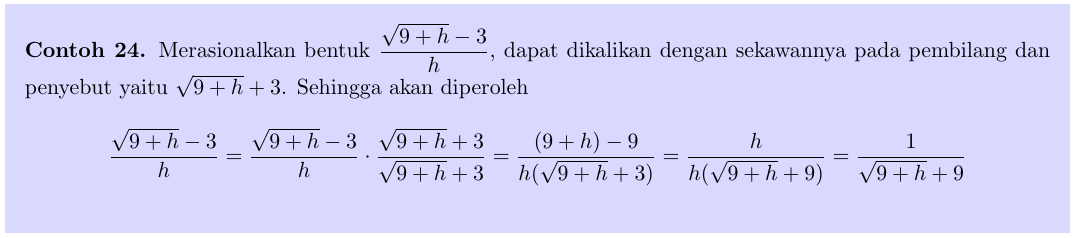
\includegraphics[width=\linewidth]{img/img42}
	\end{center}
\end{frame}

\begin{frame}{Merasionalkan Bentuk Rasional}
	\begin{center}
		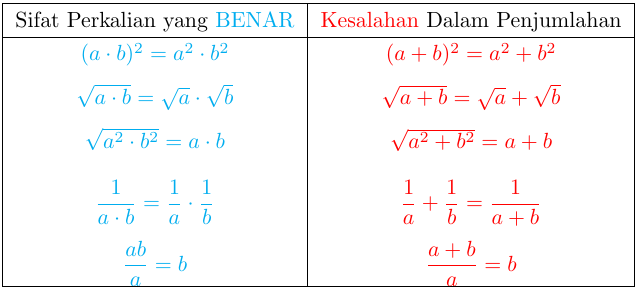
\includegraphics[width=\linewidth]{img/img43}
	\end{center}
\end{frame}

\begin{frame}
	\frametitle{Latihan Soal Operasi Bilangan Real}
	\begin{center}
		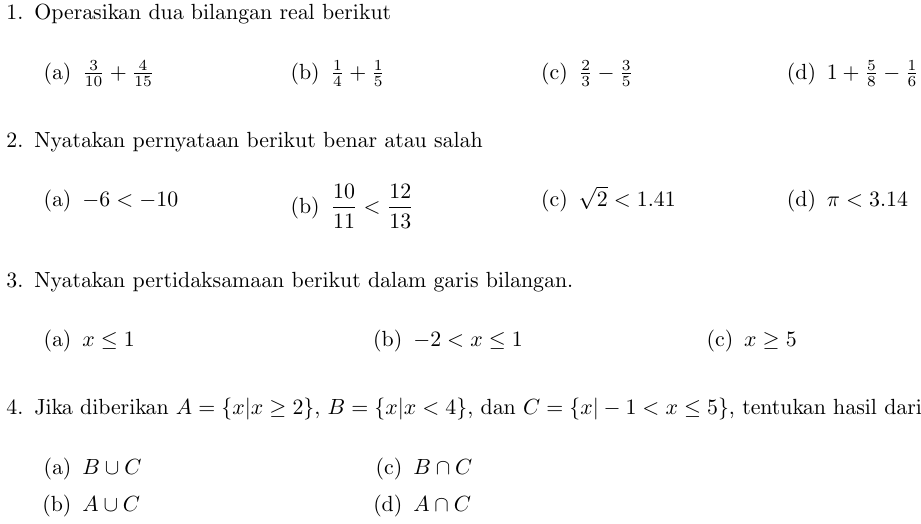
\includegraphics[width=0.8\linewidth]{img/img44}
	\end{center}
\end{frame}

\begin{frame}{Latihan Soal Operasi Bilangan Real}
	\begin{center}
		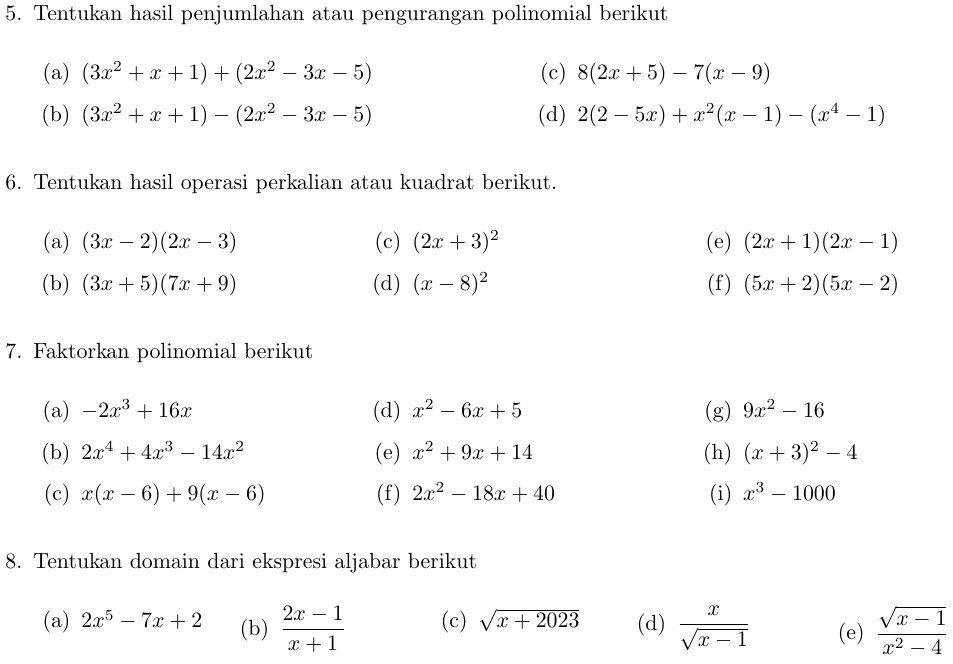
\includegraphics[width=0.8\linewidth]{img/img45}
	\end{center}
\end{frame}

\begin{frame}{Latihan Soal Operasi Bilangan Real}
	\begin{center}
		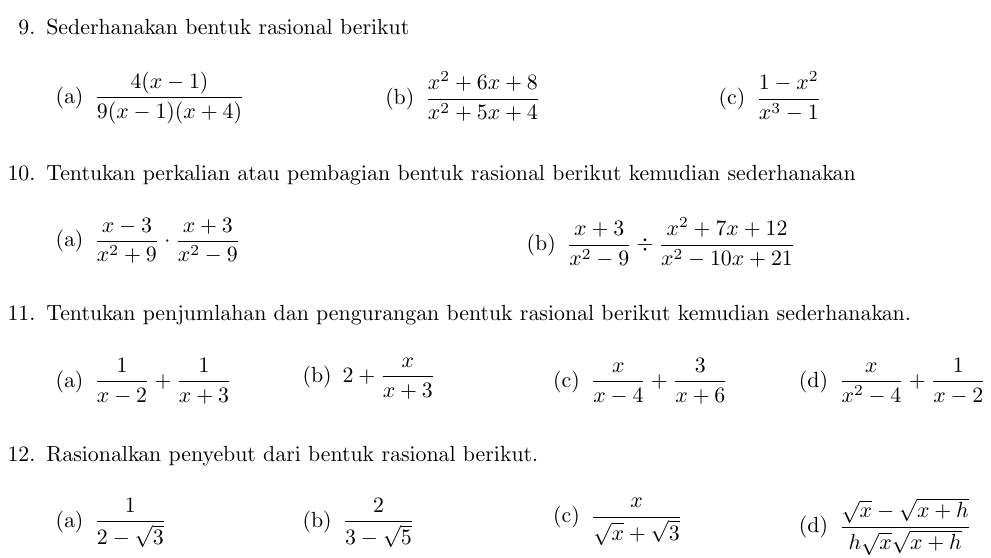
\includegraphics[width=0.8\linewidth]{img/img46}
	\end{center}
\end{frame}

\begin{frame}
	\centering
	\Huge{TUGAS}
\end{frame}

\end{document}
